\documentclass{suribt}
\title{ゲーム「2048」のプレイヤについて}
\author{金澤望生}
\eauthor{Kanazawa Nozomu}
\studentid{08-152021}
\supervisor{山口和紀 教授}
\handin{2018}{1}
\keywords{ゲームAI,機械学習}
\usepackage[dvipdfmx]{graphicx}
\usepackage{float}

\begin{document}
\maketitle

\frontmatter
\begin{abstract}
インターネットブラウザやスマートフォン上で遊ぶことのできるパズルゲーム「2048」をプレイするAIの改良を行った.改良には盤面上で最も大きな数のタイルが隅にあることを重視する独自のヒューリスティック「corner bonus」を使用した.(仮)
\end{abstract}

\tableofcontents

\mainmatter
\chapter{導入}
モチベーションや2048の基本ルール・指標について説明します.

\chapter{先行研究の紹介}
既存研究が使用している手法とプレイヤの成績について説明します.

\section{Szubert \& Jaskowski (2014)}
Szubert \& Jaskowskiは,TD学習を用いたプレイヤの訓練とnタプルネットワークを用いた価値関数の表現を組み合わせることによって,人間の知識やゲーム木探索を使用しないで十分強い2048プレイヤを実装することに成功した。
\subsection{TD学習}
TD学習の「TD」とはtemporal differenceの略であり,すなわち状態間における価値の差分を学習することによって学習器の訓練を行う手法である。2048にあてはめると,とある盤面$s'$の価値と,その盤面の1プレイ後の盤面$s'_{next}$の価値の差分を取り,これを現状定まっている$s'$に足し込んでいくことで訓練を行うことになる。TD学習にはさまざまな派生があるが,Szubert \& Jaskowskiが使用しているTD(0)学習は以下の式によって表現される:

\[
	V(s) ← V(s) + \alpha (r + V(s'') - V(s) )
\]

この式において,$V$は価値関数,$\alpha$は学習率,$r$は報酬である。学習率は計算された差分を価値関数の更新にどれほど反映するかを決定するパラメータである。

TD学習はTesauroによるバックギャモンへの適用でよく知られるようになり,碁やオセロ,チェスにおけるゲームAIの方策決定の手法として用いられるようになった。

\subsection{nタプルネットワーク}
TD学習によって盤面の評価とその学習を行うことができるが,盤面と評価値をどのように結びつけるかが問題になる。まず,2048で有り得るすべての盤面に対して評価値を与える1対1対応のルックアップテーブル(LUT)を作成することを考えると,2048で有り得る盤面の数は$(4 \times 4)^{18} \approx 4.7 \times 10^{21}$と膨大な数になり,このようなLUTを計算機上で実装することは現実的に不可能である。

そこで,一部のマスの組み合わせによる「タプル」というクラスターを作成し,さらに複数のタプルを組み合わせることで盤面を表現する手法「nタプルネットワーク」を2048に導入することが,Szubert \& Jaskowskiによって提案された。たとえば,図\ref{figure_001}のようなnタプルネットワークを実装した場合,1つのゲーム内で保持すべき重みの数は860625であり,全ての有り得る盤面に対するLUTを保持するのに対して非常に少なくて済む。

\begin{figure}[t]
	\begin{center}
	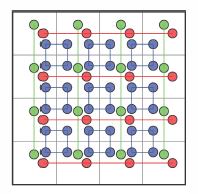
\includegraphics[width=5cm]{figure_001.png}
	\caption{nタプルネットワークの例}
	\label{figure_001}
	\end{center}
\end{figure}

nタプルネットワークはBledsoe \& Browning (1959)によりパターン認識に用いられたのが最初の採用例である。ゲームAIの分野ではJaskowski (2014)によってオセロに適用され,一定の成果が得られた。

\subsection{結果と課題}
本手法をもとに行った実験のうち,最も良い勝率を達成したプレイヤを用いて10万ゲーム中の成績を検証したところ,勝率は0.9781であり,平均スコアは100,178であった.1ゲーム中に達成されたスコアで最も良かったのは261,526であった.Szubert \& Jaskowskiによる新たな手法は探索ベースの手法よりも大幅に高速で,かつ成績が良かった.

しかしながら,この手法では「常に2048-tileを生成すること」よりも「時々16384-tileを生成すること」を重視しているため,勝率は必ずしも100\%を達成できていない.また,人間の知識を一切導入していないため,最も大きな数のタイルが盤面上の端に配置されないなど,人間の直感的な戦略とは反しているといったデメリットがあった.

\section{Wu et al. (2014)}
Wuは,Szubert \& Jaskowskiの手法を改良し,木探索を用いた先読みと組み合わせることによってさらに良いプレイヤを実装することに成功した.
\subsection{nタプルネットワークの配置の改善}
Wuは,Szubert \& Jaskowskiが考案したnタプルネットワークのうち,直線型で4タプルとして配置していたタプルを,図\ref{figure_002}(b)のように柄杓型の6タプルに変更した.これによって増える重みの数は約2倍程度であったが,この変更によってSzubert \& Jaskowskiのものよりも飛躍的に良い成績を得ることができた.なお,なぜこのようなタプルの配置が最善だと判断したのかについて,Wuは論文において言及していない.

\begin{figure}[t]
	\begin{center}
	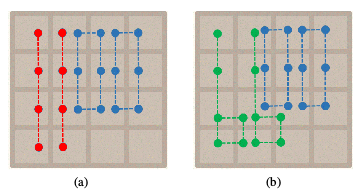
\includegraphics[width=8cm]{figure_002.png}
	\caption{Szubert \& Jaskowski(a)とWu(b)が提唱したnタプルネットワーク}
	\label{figure_002}
	\end{center}
\end{figure}

\subsection{Multi-Stage TD学習の導入}
Multi-Stage TD学習(MS-TD学習)とは,ゲームの局面に応じて異なる価値関数を保持することによって,よりそれぞれの局面に対して適切な重みを学習させることを目的とした手法である.Wuは学習のプロセスを3つのステージに分割し,ゲームプレイも同様に3つのステージに分割して行うようにした.Wuの提唱した2048におけるMS-TD学習は,以下のような手順で学習を行う.なお,「$T_{16k}$」とは「そのゲーム中で初めて16384-tileを生成することに成功した時」,「$T_{16+8k}$」とは「そのゲーム中で初めて16384-tileを生成した後に,初めて8192-tileを生成することに成功した時」のことを示す.

\begin{enumerate}
\item 第1ステージにおいては,初期盤面からゲームを始めて,価値関数が十分飽和するまで学習を行う.このステージで学習された価値関数の重みのことを「Stage-1価値関数」と呼ぶことにする.また,学習ゲーム中に$T_{16k}$を達成したなら,その時の盤面を全て保存しておく.
\item 第2ステージにおいては,第1ステージで保存した盤面からゲームを始めて,TD学習を行う.このステージで学習された価値関数の重みのことを「Stage-2価値関数」と呼ぶことにする.また,学習ゲーム中に$T_{16+8k}$を達成したなら,その時の盤面を全て保存しておく.
\item 第3ステージにおいては,第2ステージで保存した盤面からゲームを始めて,TD学習を行う.このステージで学習された価値関数の重みのことを「Stage-3価値関数
」と呼ぶことにする.
\end{enumerate}

その後,以下のような手順でゲームプレイを行う.

\begin{enumerate}
\item 盤面が$T_{16k}$を達成するまでは,Stage-1価値関数を用いてゲームプレイを行う.
\item 盤面が$T_{16k}$を達成してから$T_{16+8k}$を達成するまでは,Stage-2価値関数を用いてゲームプレイを行う.
\item 盤面が$T_{16+8k}$を達成してからは,Stage-3価値関数を用いてゲームプレイを行う.
\end{enumerate}

\subsection{Expectimax木探索}
Szubert \& Jaskowski (2014)によって,木探索ベースの2048プレイヤは強化学習で訓練したプレイヤに劣ることが示されたが,Wuは強化学習によるプレイヤに対してExpectimax木探索を補助的に組み合わせることによって,さらにプレイヤの性能を高めようと試みた.

\begin{figure}[t]
	\begin{center}
	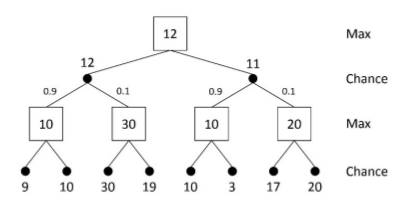
\includegraphics[width=8cm]{figure_003.png}
	\caption{Expectimax木の例 (Wu et al. (2015))}
	\label{figure_003}
	\end{center}
\end{figure}

Expectimax木探索には,MaxノードとChanceノードという2種類のノードがあり,それぞれのノードの値は子ノードから決定される.Maxノードの値は,子ノードのうち最も大きな値のノードの値となる.例えば図\ref{figure_003}の根ノードの値は12であるが,これは子ノードの「12」と「11」のうち最大の値である12を取ったものである.一方でChanceノードの値は子ノードの期待値となる.例えば図\ref{figure_003}の根ノードの子ノードの1つである「12」というノードは,0.9の確率で10となるノードと0.1の確率で3となるノードの期待値,すなわち$0.9 \times 10 + 0.1 \times 3 = 12$によって12という値が決定する.

Wuの提案においては,Maxノードの値はプレイヤがアクションを選択して遷移を行った後の盤面,Chanceノードは遷移を行った後にランダムタイルを発生させた後の盤面が与える評価値となる.例えば,ある盤面$s$(アクション選択と遷移が終わった直後の盤面とする)の評価値を深さ3のExpectimax木探索を用いて求めたい時,図hogehogeのような探索木が考えられる.$s$の盤面が分かれば,その子ノードであるランダムタイル生成後の盤面,さらにその子ノードである遷移後の盤面を求めることができる.さらに,葉ノードにあたるChanceノードの値は価値関数が与える評価値とすることで,各ノードの値を求めることができ,最終的に根ノード,すなわち評価値を求めたい盤面$s$の評価値も求められるということになる.

(図2.4. 何かいい感じの2048の探索木を自分で描画して貼る)

Expectimax木探索を用いて先読みをすることで,将来の盤面を予想してより良いアクションを選択できるようになった.これはスコアの面での成績が良くなることに繋がる一方で,maxTile=2048を達成する割合,すなわち勝率の向上にも大きな影響をもたらした.

\subsection{結果と課題}
WuによるプレイヤはSzubert \& Jaskowskiのものに比べて著しく良い成績を達成した.まずSzubert \& Jaskowskiが達成できなかった32768-tileの生成に成功し,10.9\%の確率で32768-tileを生成できるようになった.勝率に関しては1を達成,すなわち2048-tileは100\%の確率で生成できるようになり,平均スコアは328,946,最大スコアは605,752を記録した.これは当時としては1つの例外\footnote{Xiaoによる深深度先読みと人間による調整を行った評価関数を用いたプレイヤがこれにあたるが,Wuのものよりも100倍遅い:https://www.youtube.com/watch?v=JQut67u8LIg}を除き,計算機による2048プレイヤの中で最も優れた成績であった.

一方で,nタプルネットワークの形状変更やMS-TD学習のステージングについては,この研究で行なわれた調整についてこれといった根拠が述べられておらず,依然として改良の余地は残していた.特にnタプルネットワークの形状変更については,次のOka \& Matsuzakiの研究で詳しく検討されることとなった.

\section{Oka \& Matsuzaki (2016)}
Szubert \& Jaskowskiは当初図\ref{figure_001}のようなnタプルネットワークを考案していたが,このnタプルネットワークによる学習器はあまり性能が高くなく,平均スコアは10万ゲーム学習した時点で5万〜6万程度にとどまっていた.そこで,図\ref{figure_002}(a)のようなnタプルネットワークへの改良が行われ,その結果平均スコア・勝率ともに改善することができた.さらにWuはSzubet \& Jaskowskiの考案したnタプルネットワークを改良し,成績を伸ばすことができた.

しかしながら,ここまでは「タプルのサイズを大きくすると学習器の成績も良くなる」という大まかな関係しかわかっておらず,成績を最善にするnタプルネットワークはどのような形状になるのか厳密には検討されていなかった.これを厳密に検討したのがOka \& Matsuzakiである.

\subsection{nタプル単体の性能の評価}
Oka \& Matsuzakiは,まずnタプル単体の性能を網羅的に評価することを目指した.2048の盤面上でn個のタイルを選んで形成されうるnタプルの数は,表\ref{tab:ntuplesNumber}の通りとなっている.

\begin{table}[t]
	\begin{center}
		\caption{形成されうるnタプルの数}
		\begin{tabular}{l|r|r|r|r|r|r|r|r|r|r|r} \hline
		N & 3 & 4 & 5 & 6 & 7 & 8 & 9 & 10 & 11 & 12 & 13 \\ \hline \hline
		All & 77 & 252 & 567 & 1051 & 1465 & 1674 & 1465 & 1051 & 567 & 252 & 77 \\ \hline
		Connected & 8 & 17 & 33 & 68 & 119 & 195 & 261 & 300 & 257 & 169 & 66 \\ \hline
		\end{tabular}
		\label{tab:ntuplesNumber}
	\end{center}
\end{table}

ここで,Connectedとはタプル上の全てのタイルが1個以上の他のタプルの接していることを指す.Oka \& MatsuzakiはConnectedタプルのうち,十分性能が良く,なおかつ現実的にnタプルネットワークとして運用することができる$N=6$と$N=7$の場合のみ検討することとした.彼らは次に,形成されうるConnectedな6タプル68個の中からランダムに10個のタプルを選んで100万ゲームの学習を行う実験を680回\footnote{$680 \times 10 = 6800$より,全てのタプルが100回は選ばれるようにするため}繰り返し,各タプルの性能を比較可能な数値として算出した.7タプルについても同様な実験を行った.

その結果,6タプルと7タプルのうち最も優れた4つのタプルと最も劣った4つのタプルが,図\ref{figure_004}の通り明らかになった.

\begin{figure}[t]
	\begin{center}
	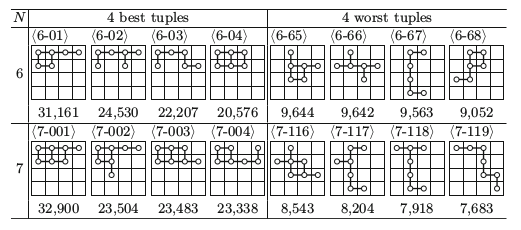
\includegraphics[width=10cm]{figure_004.png}
	\caption{最も優れている/劣っている上位4つの6タプル・7タプル (Oka \& Matsuzaki (2016))}
	\label{figure_004}
	\end{center}
\end{figure}

\subsection{nタプルネットワークに組み込むnタプルの数の検討}
6タプルおよび7タプルの性能が判明したので,性能が良い任意の数のタプルを組み合わせてnタプルネットワークを作成することが可能になった.Szubert \& JaskowskiおよびWuは4個のタプルを組み合わせてnタプルネットワークを作成していたが,Oka \& Matsuzakiは5個以上のタプルを組み合わせることを検討した.すなわち,nタプルの数が多くなればなるほどnタプルネットワーク全体としての性能も上がると思われるが,最も性能が良くなるタプルの数は何個かを明らかにするということである.

実験においては,6タプルの場合最大で上位45個,7タプルの場合最大で上位10個のタプルからnタプルネットワークを作成することとした.各nタプルネットワークに対して,600万ゲーム学習を行わせ,10,000ゲームごとに平均スコアと最大スコアを記録した.その結果が図\ref{figure_005}である.なお,mは実験を行うにあたって上位m個のnタプルを採用してnタプルネットワークを生成したことを示す.

\begin{figure}[t]
	\begin{center}
	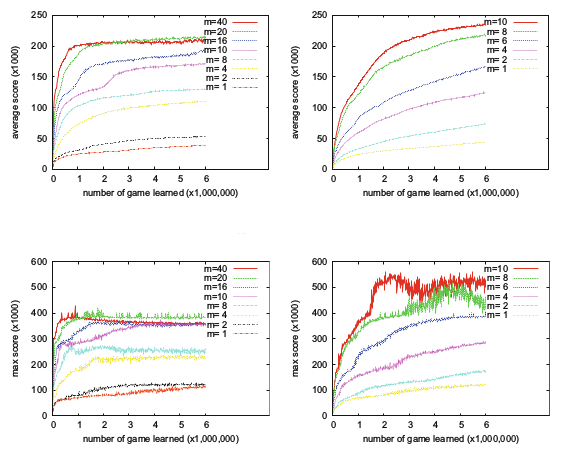
\includegraphics[width=10cm]{figure_005.png}
	\caption{成績上位タプルm個を組み合わせたタプルネットワークの実験 (Oka \& Matsuzaki (2016))}
	\label{figure_005}
	\end{center}
\end{figure}

上記の通り,実験群の中では10個の7タプルを組み合わせたタプルネットワークが最も良い成績を収めることがわかった.なお,グラフからも読み取れるが,7タプルによるネットワークに関しては600万ゲーム学習しても平均スコア・最高スコアが収束しない.そのためさらに組み合わせるタプルを増やすとさらに成績が良くなることが考えられるが,技術上の制約により$m=11$以上は実現できなかった\footnote{7タプルを組み合わせてタプルネットワークを作成する場合,重みを保持するために1個のタプルにつき1GBのメモリを消費しなければならない.Oka \& Matsuzakiが実験を行った環境はメモリが12GBしか確保できなかったため,$m=11$以上は実験を行うことが困難だったのではないかと考えられる.また,この研究においてゲーム木探索を組み込むことができなかったのもメモリの制約が原因ではないかと考えられる}.

\subsection{結果と課題}
Oka \& Matsuzakiの研究における最も良いnタプルネットワークは,勝率が0.9850,平均スコアが234,136,最高スコアが504,660という成績を残した.これはゲーム木探索を用いない計算機を用いた2048プレイヤとしては最も良い成績であった.しかしながら,ゲーム木探索を用いなかったことによりゲーム序盤では安定性を欠いてしまい,Wuが達成した勝率1を割り込む形となってしまったし,単純に2048プレイヤとしての成績を比べるとWuのものよりも平均スコア・最大スコアともに低くなっている.一方で,ゲーム木探索を採用しなかったことはプログラムの高速化という点では利があり,1秒あたり88000手の遷移を行うことができるプログラムとなった.これはWuの研究と比べて約290倍高速である.

\section{Yeh et al. (2016)}
YehはWu et al. (2014)の研究にも参画していた共同研究者で,Wuの研究の流れを引き継ぐような形で2048プレイヤの改良を行った.Wuの研究で用いたMS-TD学習の考え方,改良されたnタプルネットワーク,Expectimax木探索は引き続き用いられているため,この研究で新たに加わった要素のみを述べる.

\subsection{新たな特徴の追加}
Yehは,nタプルネットワークによる学習の他に,盤面に現れた特徴を評価関数として用いることとした.盤面の評価値には従来のnタプルネットワークによる評価値と新たに採用した特徴による評価関数の和を用い,これをTD学習で訓練した.なお,採用した特徴は以下のつである.

\begin{enumerate}
\item 大きな数が書かれたタイルの個数
\item 何も書かれていないタイルの個数
\item 異なる数が書かれた(distinct)タイルの個数
\item マージすることができるタイルのペアの組数
\item 書かれているタイルの数が$(n, 2n)$の形になっているタイルのペアの個数
\end{enumerate}

\subsection{MS-TD学習のステージングの改良}
WuはMS-TD学習を行うにあたり3ステージに分けて訓練・ゲームプレイを行っていたが,このステージの分け方をさらに細かくした.Yehによってテストされたステージングは以下の通りである.なお,$T_{x+y+zk}$という表記は,「盤面に初めて$1000x, 1000y, 1000z$のタイルが同時に現れた時」のことを指す.各タイルの数は百の位で切り捨てられて表現されている.

\begin{enumerate}
\item 4ステージ:$T_{8k}, T_{16k}, T_{16+8k}$を境界としてステージを分ける
\item 4ステージ:$T_{16k}, T_{16+8k}, T_{16+8+4k}$を境界としてステージを分ける
\item 5ステージ:$T_{16k}, T_{16+8k}, T_{16+8+4k}, T_{16+8+4+2k}$を境界としてステージを分ける
\item 6ステージ:$T_{16k}, T_{16+8k}, T_{16+8+4k}, T_{16+8+4+2k}, T_{16+8+4+2+1k}$を境界としてステージを分ける
\end{enumerate}

これらのステージングを,上から順に戦略1から戦略4とする.まず戦略1をテストした際,$T_{8k}$を境界としてステージを分けることは意味がないことがわかったため,戦略2以降では$T_{16k}$以降のステージングのみを考えることとした.戦略2から戦略4をテストした結果,平均スコアでは戦略4が最も優秀であることがわかったが,最高スコアと32678-tileの到達率では戦略3が最も優秀であった.各戦略ごとの成績は表hogehogeの通りである.

(表hogehogeをここに書きます)

以上の結果より,Yehは戦略3が最も優れたステージングだと判断し,これ以降は戦略3を用いて実験を行った.

\subsection{学習率の調整}
TD学習をより正確に行うために,まず学習率$\alpha = 0.0025$でTD学習を行った後,価値関数に大きな改善が見られなくなったと判断したら,学習率$\alpha = 0.00025$に変更して学習を続行させるようにした.

\subsection{$TD(\lambda)$の使用}
Szubert \& JaskowskiおよびWuはTD学習においてTD(0)を使用していたが,YehはTD(0.5)を用いて5ステップの報酬を平均化することとした.すなわち,

(ここに数式を書きます)

で表現される$R^{\lambda}_t$を用いてTD学習を行うようにした.

\subsection{結果と課題}
上記の改良を重ねた結果,Yehは平均スコア443,526,最大スコア793,835と非常に良い成績の学習器を訓練することに成功した.なお,32678-tileへの到達率は31.75\%,1秒あたりの遷移速度は500手であった.さらに,検証ゲーム中のある1ゲームにおいて65536-tileを生成することにも成功した.これは強化学習ベースの2048プレイヤでは当時として最も強く,Xiaoのよる深深度探索ベースのものよりも平均スコアでは優っており,Yehの方が125倍速いプログラムであった.

\chapter{本研究のアイディア}
本研究で導入しようとしている手法のアイディアについて説明します.

\chapter{提案と実装}
前章で説明したアイディアの具体的な提案とその実装方法を説明します.

\chapter{実験}
提案したアイディアの実験結果と既存研究の実験結果を比較します.

\chapter{考察と結論}
実験結果をもとに,結果の考察を行い,本研究をまとめます.

\backmatter
\chapter{謝辞}
謝辞を書きます.

\begin{thebibliography}{}
 \bibitem{}
 \bibitem{}
\end{thebibliography}

\appendix
\chapter{}
表やプログラムリストの掲載が必要になったらここに掲載します.

\end{document}
